
	This chapter will cover the necessary theoretical background and consists 
	of the following main parts:

	\begin{enumerate}
		\item Graph Theory
		\item Machine Learning on Graphs
		\item Graph Generation
    \end{enumerate}

	\section{Graph Theory}

	This section provides a brief introduction to graph theory, with a focus on
	the relevant aspects for this master thesis. The theory presented is
	primarily taken from the book "Networks: An Introduction" by Mark Newman
	\citeyearpar{Newman2010}. \\

	\noindent Graph theory is an old field of mathematics and can be traced back 
	to Leonhard Euler and the famous "Königsberg Bridge Problem"
	\citep{euler1741solutio}. The study of graphs has had a recent revival
	thanks to its useful applications in areas such as the Google algorithm
	PageRank \cite{page1999pagerank} and machine learning. Graphs are special 
	data structures as shown in Figure \ref{fig:graph}. The terms graph and network 
	are often used interchangeably and have identical meaning for the purpose
	of this master thesis. Typically, the term graph is used more commonly when 
	referring to mathematical analysis of graphs and the term network is more 
	commonly used for data science purposes. \\

	\begin{figure}[h]
		\centering
		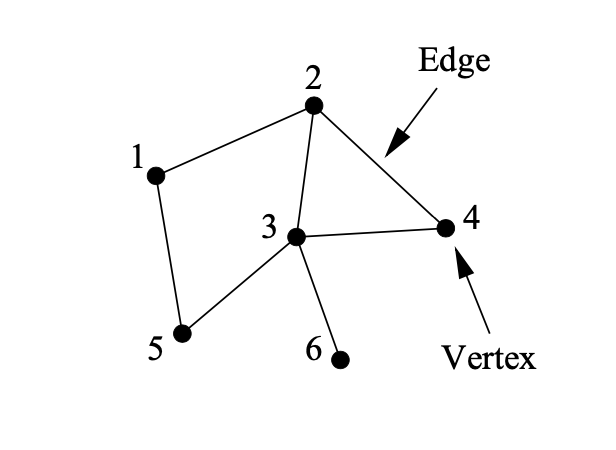
\includegraphics[width=0.5\textwidth]{graph.png}
		\caption{Example of a Graph}
		\cite[p. 111]{Newman2010}
		\label{fig:graph}
	\end{figure}
	
	\noindent The graph shown in Figure \ref{fig:graph} corresponds to an 
	undirected graph in which the connections between the vertexes are mutual. 
	In a directed graph for instance, vertex A could be connected to vertex B, 
	however vertex B need not be connected to vertex A. For the purpose of this 
	thesis, only undirected graphs are considered. Vertexes are often referred 
	to as nodes and the terms will be used interchangeably. Edges refer to the
	connections between the vertices. Edges are often also referred to as links
	and the terms will be used interchangeably as well. Graphs may have
	additional elements such as multi-edges or self-edges. Self-edges refer to
	nodes which have a looped link to itself. This can be considered as a feedback
	loop of a node on to itself. Lastly, multi-edges refer to direct node 
	connections with multiple paths. \\

	\noindent In terms of mathematical notation, graphs are typically defined
	as follows:

	\begin{equation}
		G(V,E)
	\end{equation}

	\noindent $G$ refers to the graph as an output. $V$ refers to the set of 
	vertices present in the graph and $E$ refers to edges present between the 
	vertices.

	\paragraph{Adjacency Matrix} \mbox{}\\  

	\noindent The adjacency matrix $A$ is defined as a $n \times n$ matrix, 
	where $n$ refers to the number of vertices present in the graph. Each 
	vertex is therefore recorded by a column and a row in the adjacency matrix. 
	The elements in the adjacency matrix are further typically defined as follows:

	\begin{equation}
		A_{ij} = 
			\begin{cases}
				1, & \text{if vertex $i$ and $j$ are connected by an edge} \\
				0, & \text{otherwise}
			\end{cases}
	\end{equation}
	
	\noindent For illustration, the adjacency matrix of the graph shown in 
	Figure \ref{fig:graph} is shown as follows:

	\[ A = 
	\begin{pmatrix}
		0 & 1 & 0 & 0 & 1 & 0 \\
		1 & 0 & 1 & 1 & 0 & 0 \\
		0 & 1 & 0 & 1 & 1 & 1 \\
		0 & 1 & 1 & 0 & 0 & 0 \\
		1 & 0 & 1 & 0 & 0 & 0 \\
		0 & 0 & 1 & 0 & 0 & 0  
	\end{pmatrix}
	\] 
	
	\noindent As one can see, if vertex $i$ and $j$ are connected, this is recorded with
	1 and 0 otherwise. Note, that all the elements on the $diag(A)$ are equal
	to 0. This is because there are no self-edges present in figure
	\ref{fig:graph}. Nodes with self-loops would have a 1 recorded on the
	corresponding diagonal element of the adjacency matrix. As this is an 
	undirected network, the adjacency matrix is symmetric. There are many 
	additional aspects one could mention with regard to the adjacency matrix, 
	they are however not relevant for this thesis. For additional information 
	regarding the adjacency matrix, the book "Networks: An Introduction" by 
	Mark Newman \citeyearpar{Newman2010} is highly recommended. 

	\paragraph{Degree Measures} \mbox{}\\

	\noindent An important measure for graphs are the degrees denoted by $k$ of 
	the vertices. Degrees refer to the number of edges connected to a vertex. The 
	degrees of vertex denoted by $i$ can be formulated as \citep[p. 133]{Newman2010}:

	\begin{equation}
		k_i = \sum_{j=1}^{n} A_{ij}
	\end{equation}

	\noindent For an undirected graph, edges have two ends. This is due to the 
	fact that vertices connected by an edge are mutually connected. In terms of 
	the sum of the degrees of all vertices, we can therefore write for a graph 
	with $m$ edges \citep[p. 133]{Newman2010}:

	\begin{equation}
		2m = \sum_{i=1}^{n} k_i	
	\end{equation}

	\noindent The sum of all degrees is therefore just the number of edges $m$ 
	multiplied by 2. In terms of statistical measures, the mean degree $c$ of a 
	vertex is defined as follows \citep[p. 134]{Newman2010}:

	\begin{equation}
		c = \frac{1}{n}\sum_{i=1}^{n}k_i = \frac{2m}{n}
	\end{equation}

	\noindent In order to define the connectance or density of a graph, we must
	first observe, that the maximum number of edges is given by \citep[p. 134]{Newman2010}:

	\begin{equation}
		{n \choose 2} = \frac{1}{2}n(n-1)
	\end{equation}

	\noindent The density $\rho$ can therefore be written as \citep[p. 134]{Newman2010}:

	\begin{equation}
		\rho = \frac{m}{{n \choose 2}} = \frac{2m}{n(n-1)} = \frac{c}{n-1}
	\end{equation}

	\noindent Note, that the density $\rho$ lies strictly between 
	$0 \leqslant \rho \leqslant 1$. In addition, for sufficiently large graphs,
	one can approximate $\rho = \frac{c}{n}$. 

	\paragraph{Eigenvector Centrality} \mbox{}\\

	\noindent The degrees of a vertex shown in the previous section already 
	correspond to the simplest form of centrality measures. The issue with this 
	measure however is, that the every neighbor of vertex $i$ are valued the same. 
	This is a problem, as not all neighbors are of equal importance due to:

	\begin{enumerate}
		\item Number of neighbors
		\item Importance of neighbor
		\item both
	\end{enumerate}

	\noindent There are many different alternative centrality measures which
	can consider the factors listed above such as eigenvector centrality, Katz
	centrality or PageRank
	\citep{katz1953new,page1999pagerank,landau1895relativen,Newman2010}. As we 
	are only dealing with simple undirected graphs, eigenvector centrality will 
	suffice, where the other mentioned methods are adaptations to the 
	eigenvector centrality. \\

	\noindent Eigenvector centrality gives all vertices a score proportional to
	the sum of the scores of its neighbors. This is a procedure in which
	typically the initial centrality $x_i$ of vertex $i$ is guessed to be 1
	$\forall \; i$. This can be used to calculate the centralities of the
	neighbors of $i$ which is denoted as $x_{i}'$. We can thus write
	\citep[p. 169]{Newman2010}:

	\begin{equation}
		x_i' = \sum_{j}A_{ij}x_j
	\end{equation}

	\noindent In matrix form:

	\begin{equation}
		x' = Ax
	\end{equation}

	\noindent This process is repeated $t$ times to provide better estimates
	\citep[p. 170]{Newman2010}:

	\begin{equation}
		x(t) =  A^tx(0)
	\end{equation}

	\noindent Where $x(0)$ is a linear combination of \citep[p. 170]{Newman2010}:

	\begin{equation}
		x(0) =  \sum_{i}c_{i}v_{i}
	\end{equation}

	\noindent $v_i$ corresponds to the eigenvectors of the adjacency matrix $A$
	and $c_i$ corresponds to an appropriately chosen constant. Therefore we can
	write \citep[p. 170]{Newman2010}:

	\begin{equation}
		x(t) =  A^t \sum_{i}c_{i}v_{i} = \sum_{i} c_i k_i^t v_i = 
		k_i^t \sum_{i} c_i \left[\frac{k_i}{k_1}\right]^t v_i
	\end{equation}

	\noindent In the above equation, $k_i$ correspond to the eigenvalues of $A$, 
	the adjacency matrix. $k_1$ corresponds to the largest eigenvalue of $A$.
	As $\frac{k_i}{k_1} < 1, \; \forall \; i\neq 1$ , the term is decaying as 
	$t \rightarrow \infty$. The centralities $x$ can therefore be written
	as fulfilling following condition \citep[p. 170]{Newman2010}:

	\begin{equation}
		Ax = k_1 x	
	\end{equation}

	\noindent Lastly, the eigenvector centrality is defined as \citep[p. 170]{Newman2010}:

	\begin{equation}
		x_i = k_{1}^{-1} \sum_{j} A_{ij}x_j 
	\end{equation}

	\paragraph{Closeness Centrality} \mbox{}\\

	\noindent Closeness centrality, $C_i$, is defined as the average distance 
	from a vertex to the other vertices. This centrality measure is defined as 
	follows \citep[p. 182]{Newman2010}:

	\begin{equation}
		C_i = \frac{1}{l_i} = \frac{n}{\sum_{j}d_{ij}}
	\end{equation}

	\noindent In this measure, central vertices exhibit high closeness 
	centrality and are therefore closer connected to other vertices compared to 
	vertices with low closeness centrality. $l_i$ refers to the average of the 
	geodesic distances $d_{ij}$ of vertex $i$.

	\paragraph{Betweenness Centrality} \mbox{}\\

	\noindent This centrality measures to which extent a vertex lies on paths 
	between other vertices. For instance, a bottle neck vertex would exhibit a 
	large betweenness centrality as many, if not all nodes must pass through it. 
	More formally, betweenness centrality, $x_i$, is defined as 
	\citep[p. 187]{Newman2010}:

	\begin{equation}
		x_i = \sum_{st} \frac{\eta_{st}^i}{g_{st}}
	\end{equation}

	\noindent In the above equation, $\eta_{st}^i$ refers to the number of 
	geodesic paths from $s$ to $t$ which pass through vertex $i$. Further,
	$g_{st}$ is defined as the number of geodesic paths between vertex $s$ and
	$t$. \\

	\noindent In order to allow for better comparison of betweenness
	centrality, it is often standardized by the number of connected vertex
	pairs $s$ and $t$ denoted as  $\eta^2$. The betweenness centrality
	can therefore be expressed as \citep[p.190]{Newman2010}:

	\begin{equation}
		x_i = \frac{1}{\eta^2}\sum_{st} \frac{\eta_{st}^i}{g_{st}}
	\end{equation}

	\noindent With this measure, the betweenness centrality is within the range
	$0\leqslant1$

	\section{Machine Learning on Graphs}

	\noindent Graph structures are special in that the data points in a graph 
	have connections with each other. A practical example for this are social 
	networks. In a social network, the profiles of "Peter" and "Paul" might be 
	connected because "Peter" and "Paul" are friends. In addition, "Paul" and 
	"Peter" can only ever reach each-other if they are directly or perhaps 
	indirectly connected. This aspect is unique to graph or network data and 
	provides both additional information as well as additional complexity to 
	graph data. This property does not allow for comparing nodes in a graph in 
	terms of euclidean distances as only connected nodes can reach each-other. 
	For the purpose of this thesis, machine learning on graphs will be 
	categorized into two categories:

	\begin{enumerate}
		\item Graph representation learning with subsequent downstream machine
			learning
		\item Graph neural networks
	\end{enumerate}
	
	\noindent Graph representation learning refers to models in which node
	embeddings of a graph are learned. Specifically, this approach yields
	vector representations of the nodes in a graph for which distance measures
	such as Euclidean distances can be measured. These node vector
	representations can then be used as feature data for standard machine
	learning methods. Graph neural networks can perform both graph representation
	learning as well as machine learning tasks within the same model/step. This
	combination is what makes graph neural networks stand out compared to other
	graph representation learning methods. \\

	\noindent In the following subsections, the theory for graph representation 
	learning models as well as graph neural networks are introduced. 

	\subsection{Graph Representation Learning}

	The aim of graph representation learning is to generate node embeddings in 
	the form of a $d$-dimensional vector representation. The resulting vector 
	embeddings can then be used for "standard" machine learning applications. 
	A graphical representation of this task is shown in figure 
	\ref{fig:embedding}.

	\begin{figure}[h]
		\centering
		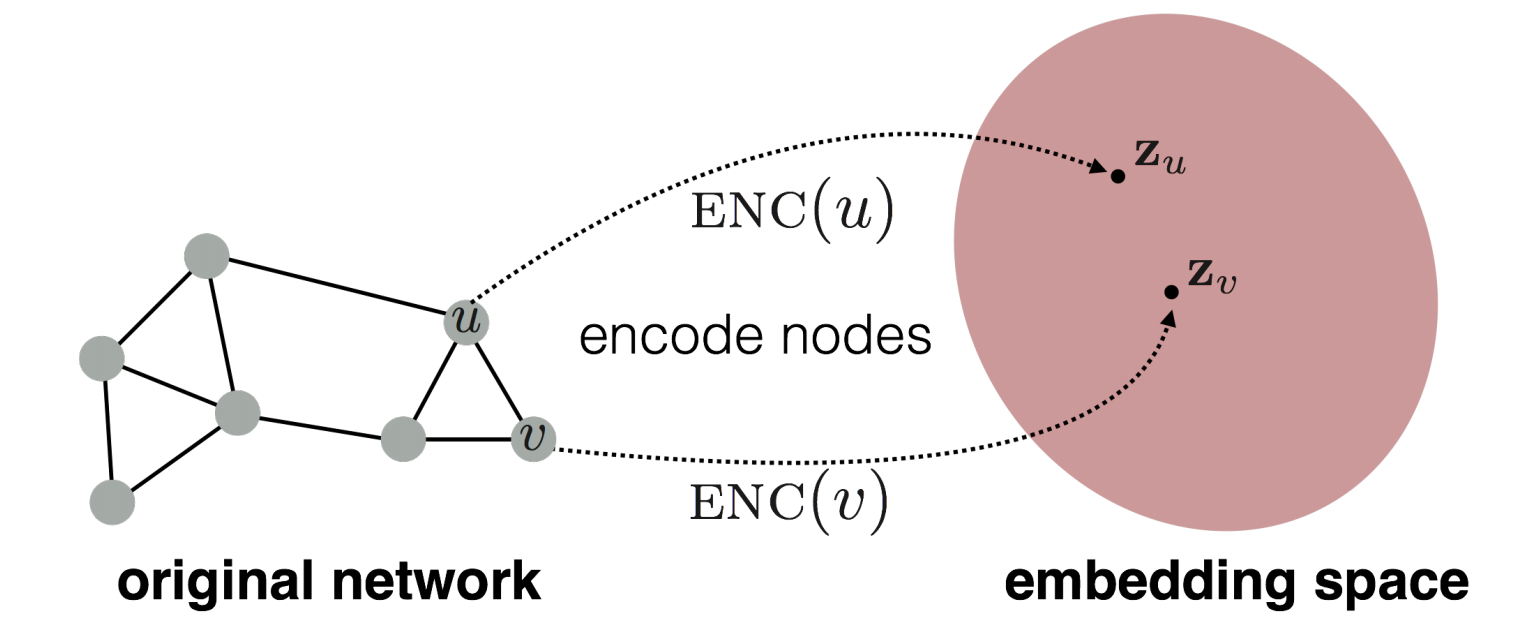
\includegraphics[width=0.8\textwidth]{embedding.png}
		\caption{Network Embedding}
		\cite{leskovec2021lecture}
		\label{fig:embedding}
	\end{figure}

	\noindent To generate node embeddings of a graph, one has to define an
	encoder which transforms nodes in a graph into their embedding space as
	shown in figure \ref{fig:embedding}. The nodes must be embedded in such a
	manner that similar nodes in the graph are also embedded closely in the 
	embedding space. A common measure for similarity is to find vector embeddings 
	$z$ of nodes $u$ and $v$ such that \citep{leskovec2021lecture}:

	\begin{equation}
		z_u^Tz_v \approx similarity(u,v)
	\end{equation}

	\noindent The dot product of the two node embedding vectors should thus
	approximately equal the similarity of the corresponding nodes in the
	graph. There are different approaches for defining node similarity. Graph 
	factorization was introduced as an early solution 
	\citep{ahmed2013distributed}. More recent and more successful approaches 
	include methods which make use of random walks. In the context of random
	walks, similarity is defined as \citep{leskovec2021lecture}:

	\begin{equation}
		z_u^Tz_v \approx \text{Probability that node $u$ and $v$
								co-occur on a random walk over the graph}
	\label{eq:random_similartiy}
	\end{equation}

	\noindent The methods DeepWalk \citep{perozzi2014deepwalk} and its 
	generalization Node2Vec \citep{grover2016node2vec} successfully apply the
	similarity measure shown in equation \ref{eq:random_similartiy}. Another 
	noteworthy method called LINE \citep{tang2015line} also makes use of random
	walk co-occurrences as its similarity measure. In order to remain focused,
	only DeepWalk and Node2Vec are considered for this thesis. These two models
	are well suited for the given task and are among the most popular graph
	representation learning methods. \\

	\noindent DeepWalk and Node2Vec make use of methods which have its origin in 
	natural language processing (NLP). Specifically they makes use of the 
	Skip-Gram model \citep{mikolov2013efficient,mikolov2013distributed}. The 
	Skip-Gram model is a core component of DeepWalk and Node2Vec, which is why 
	it is explained in detail before proceeding to DeepWalk and Node2Vec. \\

	\noindent In NLP words are one-hot encoded as inputs for the Skip-Gram model 
	which learns vector representations of the input words. Similarly, nodes in 
	a network can be thought of as words in a NLP framework. The aim of the
	Skip-Gram model is then to predict the context of the input word by
	predicting its neighboring words in a sentence. A basic overview of the 
	Skip-Gram model is provided in figure \ref{fig:skip_gram}. 

	\begin{figure}
		\centering
		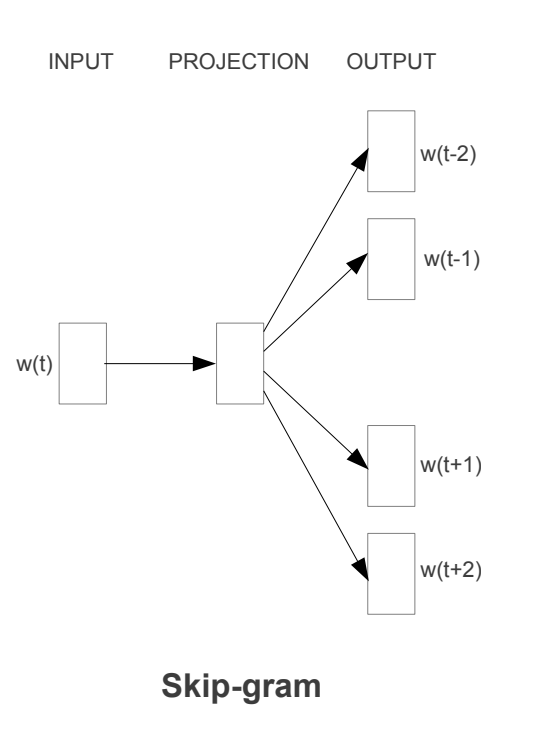
\includegraphics[width=0.4\textwidth]{skip_gram.png}
		\caption{Skip-Gram Architecture}
		\cite[p. 5]{mikolov2013efficient}
		\label{fig:skip_gram}
	\end{figure}

	\noindent The basic layout shown in figure \ref{fig:skip_gram} depicts the
	high level procedure of the skip-gram model. To make this model more
	specific, the input corresponds to the one-hot encoded vector at row $t$ of
	the input matrix $W$ with dimensions $T \times T$, where every row 
	corresponds to a one-hot encoded word. $W(t)$ is linearly passed to the
	projection, which involves calculating the dot product of $W(t)$ with the 
	weight matrix $\Phi$ which has dimensions $T \times D$. $D$ refers to the
	number of dimensions which are to be included in the projection vector $h$ 
	and is a hyper parameter. The projection vector $h$ is then linearly passed
	again with another weight matrix $\Psi$ which has dimensions $D \times T$.
	This creates the output vector $u$ which is then used to predict the correct
	context word $c$ from the vocabulary of $C$ number of context words. To do 
	so, the training target is set to maximize the average $\log$ probability 
	of the correct context word for every input word $W(t)$. More formally 
	\citep[p. 2]{mikolov2013distributed}:

	\begin{equation}
		\frac{1}{T}\sum_{t=1}^{T}\sum_{-c \leqslant j \leqslant c,j\neq0}\log
		p(w_{t+j}\mid w_{t})
		\label{eq:skip_traintarget}
	\end{equation}

	\noindent To calculate the probability of the context word given the input
	word $W(t)$, the Softmax function is applied to the output layer $u$ in the 
	manner shown by Mikolov et al. (\citeyear[p. 3]{mikolov2013distributed}). This 
	calculates a normalized probability for every context word given $W(t)$. To 
	formalize this in terms of a loss function, the training target shown in 
	equation \ref{eq:skip_traintarget} can be rewritten as follows:

	\begin{equation}
		\begin{split}
			\mathcal{L} =& - \log p(w_{t-c},w_{t-c+1},\dots,w_{t+c-1},w_{t+c}\mid w_{t})\\
			=& - \log \prod_{c=1}^{C}\frac{\exp(u_{c,j_{c}^{*}})}{\sum_{j'=1}^{T}
			\exp(u_{j'})}\\
			=&	- \sum_{c=1}^{C} u_{j_{c}^{*}} + C \cdot \log
								\sum_{j'=1}^{T} \exp(u_{j'})
	\end{split}
	\end{equation}

	\noindent The notation was slightly adjusted, where $u_{j_{c}^{*}}$ refers
	to the index of the output vector $u$ which corresponds to the actual
	context word $c$ given the input word $W(t)$. In turn, 
	$\sum_{j'=1}^{T}\exp(u_{j'})$ is a summation over all exponentiated output 
	representations $u_{j'}$ of all $T$ number of words given the input word 
	$W(t)$. The calculated loss is then used to update the trainable model 
	parameters $\Phi$ and $\Psi$ using gradient descent via a backward 
	propagation function analogues to what is used for standard neural 
	networks. The desired output of the Skip-Gram model is the weight matrix
	$\Phi$ which once the model is sufficiently trained, corresponds to the
	vector representation or embeddings of the input words. \\

	\noindent The same principle shown in the Skip-Gram model can be applied
	to graphs in a modified version. First, nodes in graph can be one-hot
	encoded the same way as words. This means, that nodes can be used as input
	data in a similar fashion as words. Based on this idea, DeepWalk by
	\cite{perozzi2014deepwalk} achieved a big breakthrough for graph
	representation learning. The DeepWalk algorithm builds on top of the 
	Skip-Gram model and uses fixed-length random walks for learning the node 
	vector embeddings. To provide a better overview of the DeepWalk algorithm, 
	the pseudo-code is presented in algorithm \ref{algo:DeepWalk} \& 
	\ref{algo:SkipGram} \citep[p. 704]{perozzi2014deepwalk}.
	
	\begin{algorithm}
		\scriptsize
		\SetAlgoLined
		\KwIn{graph $G(V,E)$}
		window size $w$\\
		embedding size $d$\\
		walks per vertex $\gamma$\\
		walk length $t$\\
		\KwOut{matrix of vertex representations $\Phi \in \mathbb{R}^{\mid V
		\mid \times d}$}
		\nl Initialization: Sample $\Phi$ from $\mathcal{U}^{\mid V
		\mid \times d}$ \\
		\nl Build a binary Tree $T$ from $V$ \\
		\nl \For{$i=0$ to $\gamma$}{
		\nl		$\mathcal{O}$ = Shuffle($V$) \\
		\nl		\ForEach{$v_i \in \mathcal{O}$}{
		\nl			$\mathcal{W}_{vi} = RandomWalk(G,v_i,t)$\\
		\nl			SkipGram($\Phi,\mathcal{W}_{vi}, w$)
				}
			}
		\caption{DeepWalk($G,w,d,\gamma,t$)}
		\label{algo:DeepWalk}
	\end{algorithm}
	
	\begin{algorithm}
		\scriptsize
		\SetAlgoLined
		\nl \ForEach{$v_j \in \mathcal{W}_{vi}$}{
		\nl		\ForEach{$u_k \in \mathcal{W}_{vi}[j-w:j+w]$}{
		\nl			$J(\Phi) = - \log \Pr(u_k \mid \Phi(v_j))$\\
		\nl			$\Phi = \Phi - \alpha * \frac{\partial J}{\partial \Phi}$
				}
			}
		\caption{SkipGram($\Phi,\mathcal{W}_{vi},w$)}
		\label{algo:SkipGram}
	\end{algorithm}
	
	\vspace{5mm}
	
	\noindent The DeepWalk algorithm shows, that for every node $v\in G$ a
	fixed length random walk is created. Every node on the random walk is used
	as a one-hot encoded input for the Skip-Gram model. The context nodes of the
	input node correspond to the input nodes' neighbors on the random walk 
	within the window size distance $w$. This procedure is repeated for $\gamma$ 
	number of random walks which in turn conclude one training epoch. 

	Lastly, the DeepWalk
	algorithm often uses more efficient approximation methods such as
	hierarchical Softmax which makes use of a binary tree or negative sampling.
	Both approximation methods are outlined in the paper by
	\cite{mikolov2013distributed}. \\

	\noindent This is in principle the model which will be used to find the node
	embeddings. In the application, the Node2Vec algorithm by will be employed. 
	Node2Vec is a generalization of the DeepWalk algorithm and allows for the deployment of
	biased random walks. In particular, it allows to set probabilities as to
	whether the random walk is biased towards breadth-first (BFS) search or
	depth-first search (DFS). Depending on the network structure, setting an
	appropriate bias can greatly improve the quality of the embeddings. If no
	bias towards BFS or DFS is set, an unbiased random walk is employed which is when
	the Node2Vec algorithm corresponds to the DeepWalk algorithm. More
	precisely, this occurs when the search bias $\alpha = 1$ with $p=q=1$ as
	outlined in the Node2Vec paper \citep[p. 860]{grover2016node2vec}. The results
	revealed, that an unbiased random walk embedded the nodes very well. For
	that reason the Node2Vec algorithm is not explained in further detail as
	the relevant parts are covered by the simpler and reader friendlier 
	DeepWalk algorithm. \\

	\noindent The resulting node vector embeddings can then be used for downstream
	machine learning tasks. An additional benefit of graph representation
	learning is that the nodes can be encoded into an arbitrary number of
	dimensions. In this sense, graph representation learning can be used as a
	powerful dimensionality reduction strategy. Further, the node embedding vectors
	correspond to the features used in the downstream machine learning tasks.
	The values of the features were learned automatically using the DeepWalk or
	Node2Vec algorithm. This approach directly takes care of the otherwise
	tedious feature selection process. With this approach, only the number of
	features needs to be defined in terms of feature selection. This is a large
	advantage and can save a lot of time when working with graphs. 

	\subsection{Graph Neural Networks}

	This section will provide an overview regarding the theory about Graph
	Neural Networks (GNN). Within the family of GNNs, there are a myriad of
	different methods available and every few months new methods are being
	published. GNNs currently enjoy a large popularity and benefit from a large
	research output. This thesis will focus on two popular and established GNN
	approaches which are:

	\begin{enumerate}
		\item Graph Convolutional Networks
		\item GraphSage
	\end{enumerate}
	
	\noindent Before presenting the two above mentioned methods, a general
	overview of the GNN framework is given. First the required setup is
	defined \citep{leskovec2021lecture}:

	\begin{itemize}
		\item $G(V,E)$ is a graph with a set of vertices and edge connections
		\item $V$ is a set of vertices
		\item $A$ is the adjacency matrix graph $G$
		\item $X \in \mathbb{R}^{\mid V\mid \times F}$ is the matrix of node
			features
		\item $v$ is a node $\in V$ and $\mathcal{N}(v)$ is the set of
			neighbors of $v$
	\end{itemize}

	\noindent If there are no node features present, $X$ can for instance be
	defined as a one-hot encoded vector. A naïve approach would be to join the 
	adjacency matrix with the feature matrix as the input for a artificial
	neural network. The problem with this approach is, that the input is not order 
	invariant and the model cannot be applied to graphs of different sizes
	\citep{leskovec2021lecture}. \\


	\noindent Modern GNNs have overcome this problem by drawing inspiration from 
	Convolutional Neural Networks (CNN) and its famous filtering mechanism as 
	outlined by \cite{krizhevsky2012imagenet}.
	CNNs typically work with grid structured input data such as pixels of
	images. The convolutional filter then samples the input grid using a
	filter with a specified size (e.g. $3\times3$ grid filter). Similarly GNN
	sample a graph using the node neighbors $\mathcal{N}(v)$ of node $v$ as a
	filter. The filter can then be fine tuned in the sense of how many $k$-hops
	of neighbors to consider (e.g. 1-hop: immediate neighbors of $v$, 2-hop:
	include neighbors of $v$'s neighbors etc.). In terms of implementation, the
	number of $k$-hops is set by the number of graph convolutional layers
	included in the GNN model. A graphical illustration of this mechanism is 
	shown in figure \ref{fig:GNN_structure}. \\

	\begin{figure}
		\centering
		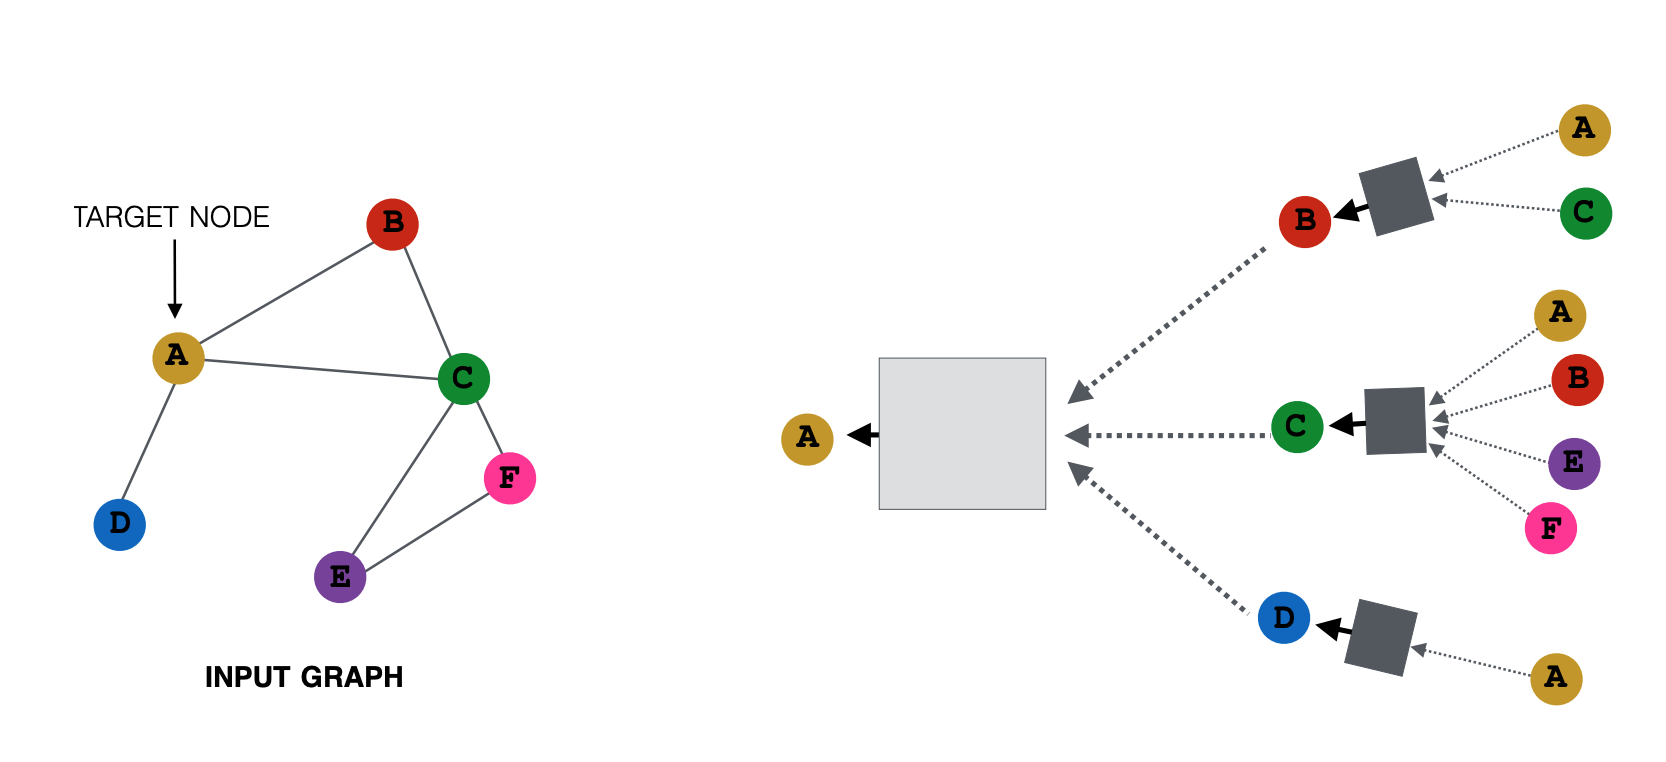
\includegraphics[width=0.8\textwidth]{GNN.png}
		\caption{GNN Structure}
		\cite{leskovec2021lecture}
		\label{fig:GNN_structure}
	\end{figure}


	\noindent The GNN Structure outlined shows an example of a 2-hop or 2 layer GNN. 
	The 1-hop convolutional layer considers the neighboring nodes of the target node A. 
	The 2-hop layer considers the neighbors of node A's neighbors. Note, that the 
	target node A is included as an input node in the 2-hop layer. This is reasonable 
	as node A itself is also a neighboring node to it neighbors. Further, node 
	A is also a determining factor for its neighbors. Taking the example shown in
	figure \ref{fig:GNN_structure}, the challenge for the GNN is to find node
	embeddings based on local network neighborhoods
	\citep{leskovec2021lecture}. The node embeddings at layer 0 correspond to
	the features of the input nodes where $X = H^{(0)}$. A typical procedure
	for a GNN model is outlined in algorithm \ref{algo:GNN_struct}
	\citep{hamilton2017inductive,leskovec2021lecture,you2020design}.
	

	\begin{algorithm}
		\scriptsize
		\SetAlgoLined
		\KwIn{Graph $G(V,E)$;}
		\myinput{input features $\{x_v,\forall v \in V\}$;}
		\myinput{node labels $\{y_v, \forall v \in V\}$;}
		\myinput{training set $\mathcal{T}\subseteq V$;}
		\myinput{depth/layers $K$ with parameters $\Theta^{k} =
		\{W^{k},B^{k}\},\forall k \in \{1\dots K\}$} 
		\myinput{non-linearity $\sigma$;}
		\myinput{differentiable aggregator functions $AGGREGATE_k,\forall k \in
					\{1,\dots,K\}$;}
		\myinput{neighborhood function $\mathcal{N}:v\rightarrow 2^{V}$;}
		\myinput{loss function $\mathcal{L}$ such as cross entropy $CE$;}
		\myinput{learning rate $\alpha$}
		\KwOut{Vector representations $z_v, \forall v\in V$}
		\nl Initialize layer specific $W^{k}$ from $\mathcal{U},\forall k \in 
			\{1,\dots,K\}$\;
		\nl Initialize layer specific $B^{k}$ from $\mathcal{U},\forall k \in
			\{1,\dots,K\}$\;
		\nl $h_{v}^{0} = x_{v},\forall v \in \mathcal{T}$\\
		\nl \For{Number of epochs}{
		\nl \For{$k=1\dots K$}{
		\nl		\For{$v\in \mathcal{T}$}{
		\nl			$h_{\mathcal{N}(v)}^{k} \leftarrow AGGREGATE_k\left(
					{h_{u}^{k-1},\forall u \in\mathcal{N}_{k}(v)}\right)$\;
		\nl			$h_{v}^{k} \leftarrow\sigma \left(W^{k}\cdot 
							CONCAT(h_{v}^{k-1},h_{\mathcal{N}(v)}^{k})\right)$\;
					}		
		\nl		$h_{v}^{k} \leftarrow h_{v}^{k}/\lVert h_{v}^{k}\rVert_{2},
										\forall v \in \mathcal{T}$	
   			}
		\nl $z_v = h_{v}^{K},\forall v \in \mathcal{T}$\;
		\nl $\mathcal{L}(\Theta)=\sum_{(z_{v},y_{v})\in\mathcal{T}}CE(y_{v},z_{v})$\;
		\nl $\Theta = \Theta - \alpha\cdot \frac{\partial\mathcal{L}}{\partial\Theta}$
		}
		\caption{Typical GNN algorithm for training data}
		\label{algo:GNN_struct}
	\end{algorithm}


	\noindent Algorithm \ref{algo:GNN_struct} is not meant to be considered as
	a complete overview and should be rather regarded as an example of a typical 
	GNN structure. GNNs are flexible in that a myriad of modifications can be 
	added to the GNN layers similar to the possibilities of CNNs or ANNs. The 
	defining features of different GNN methods usually involve the selection of 
	different message passing methods and aggregation strategies. An excellent 
	overview regarding the design space for GNNs is provided in the articles by
	\cite{you2020design} and \cite{zhou2020graph}.
	Of course there are exceptions and alternative procedures exist. The GNN 
	methods evaluated in this thesis and most successful GNNs however tend to 
	follow a variation of the structure shown in algorithm 
	\ref{algo:GNN_struct}.  \\

	\noindent In terms of interpretation, the output of the first GNN layers in
	figure \ref{fig:GNN_structure} (gray boxes) corresponds to the hidden layer 
	representations of the direct neighbors of target node A and the output of 
	the final GNN layer corresponds to the node embedding of the target node A. 
	This should sound familiar when comparing this approach to the graph 
	representation learning approach outlined in the previous section. 
	GNNs can indeed be used for unsupervised learning tasks such as finding node 
	embeddings such that similar nodes are embedded close together. Good
	examples for this is shown in the papers regarding Graph Convolutional
	Networks by \cite{kipf2016semi} and GraphSage by
	\cite{hamilton2017inductive}. As shown in algorithm \ref{algo:GNN_struct},
	GNNs can be applied directly to a supervised learning task. In order to
	avoid redundancy with the graph representation learning strategies
	introduced previously, the GNNs will be applied in a supervised learning
	context. GNNs are powerful tools for unsupervised learning for tasks such
	as clustering or graph representation learning \citep{zhou2020graph}. While
	GNNs are possibly more efficient for graph representation learning 
	\citep[p. 12-13]{kipf2016semi}, the results are unlikely to differ 
	significantly and is not the focus of this thesis. The aim is to use GNNs
	in a supervised learning setting as it hopefully provides superior results
	for a given classification task. In the following paragraph the first GNN 
	method of interest is presented. 


	\subsubsection{Graph Convolutional Networks}
	
	\noindent The Graph Convolutional Network (GCN) was introduced by 
	\cite{kipf2016semi} and makes use of simplified spectral graph
	convolutions. The author Thomas Kipf \citeyearpar{kipf2016online} provides 
	excellent explanations on his website which is used as inspiration for
	presenting the theory. As outlined, GNNs typically differ with regards to
	the type of message passing and aggregation strategy. GCN make us of the
	following forward propagation method \citep[p. 2]{kipf2016semi}:

	\begin{equation}
		H^{(l+1)} = \sigma\left(\tilde D^{-\frac{1}{2}}\tilde A \tilde
		D^{-\frac{1}{2}}H^{(l)}W^{(l)}\right)
		\label{eq:GCN}
	\end{equation}
	
	\noindent The variables in equation \ref{eq:GCN} are defined as follows:

	\begin{itemize}
		\item $H^{l}\in\mathbb{R}^{N \times D}$ refers to the embedding matrix
			at layer $l$ where $N$ refers to the number of nodes $\mid V \mid$
			and $D$ refers to the number of embedding dimensions. The input
			embedding matrix is set equal to the feature matrix, $H^{(0)}=X$.
		\item $W^{l}$ refers to the trainable and layer specific weight matrix
			for the linear message passing employed in the GCN model.
		\item $\tilde A = A + I_N$ where $A$ is the adjacency matrix of the
			input graph $G$. The identity matrix is added so that self-loops
			are considered. This is necessary as the target node of every layer
			is considered in the aggregation process as previously outlined.
		\item $\tilde D_{ii} = \sum_{j}\tilde A_{ij}$ is a diagonal matrix
			containing the degree distributions of the modified adjacency
			matrix $\tilde A$.
		\item $\sigma(\cdot)$ refers to an activation function such as ReLu or
			Softmax.
	\end{itemize}

	\noindent To provide a better overview, the compact notation shown in 
	equation \ref{eq:GCN} is expanded in the following equation for one GCN
	layer \citep{Dubois2019}:

	\begin{equation}
		h_{ij}^{(l)} = \sigma\left(\sum_{(i,j)\in
		\mathcal{N}(v)}\frac{\tilde a_{ik}h_{kj}^{(l-1)}}{\sqrt{\tilde
d_{k,k}\tilde d_{i,i}}} W^{(l)}\right)
		\label{eq:GCN_expand}
	\end{equation}
	
	\noindent In Equation \ref{eq:GCN_expand} $h_{ij}^{(l)}$ refers to the 
	hidden layer representation of node $i$ at layer $l$ considering the set of
	neighbors $j$. $h_{kj}^{(l-1)}$ corresponds to the hidden layer
	representation of node $k$ at layer $l-1$ which is part of the set of 
	neighbors $j$. In terms of filtering strategy, $(i,j) \in \mathcal{N}(v)$. 
	This means that both set of nodes $i$ and $j$ are neighbors of the target 
	node $v$ at layers $l$ and $(l-1)$ respectively. Linear message
	passing is then performed for every neighbor in $j$ at layer $l-1$. The node 
	in the graph $G$ at position $\tilde a_{ik}$ of the modified adjacency matrix 
	selects the nodes for which a connection between $h_{ij}^{(l)}$ and
	$h_{kj}^{(l-1)}$ exists. The embeddings $h_{kj}^{(l-1)}$ of the selected 
	nodes are normalized by the symmetric degree distributions of the previous 
	hidden layer node $\tilde d_{k,k}$ and the new hidden layer node $\tilde d_{i,i}$.
	Afterwards the normalized embeddings are message passed by multiplying it
	with the shared weight matrix $W^{(l)}$. Lastly, the sum of the received
	messages is taken in terms of aggregation strategy and the resulting
	aggregate is passed through the activation function to yield $h_{ij}^{(l)}$.
	Note, that the aggregation strategy involves taking a weighted sum thanks
	to the symmetric normalization. \\

	\noindent The detailed explanations given above show the procedure for
	one layer of a GCN. Returning now to compact notation, this procedure can be
	expanded for two or more GCN layers. First, the notation is further
	simplified by defining $\hat A = \tilde D^{-\frac{1}{2}}\tilde A \tilde
	D^{-\frac{1}{2}}$. An example of a two-layer GCN is then given as follows 
	where $Z$ refers to the embedding or output of the target node 
	\citep[p. 3]{kipf2016semi}:

	\begin{equation}
		Z = f(X,A) = \text{softmax}\left(\hat A \;\text{ReLu}\left(\hat A X
		W^{(0)}\right)W^{(1)}\right)
	\label{eq:GCN_forward}
	\end{equation}

	\noindent Finally, the model parameters are updated analogues to the
	procedure outlined in algorithm \ref{algo:GNN_struct}. The main distinctive
	feature for the GCN is the differing forward propagation procedure. 

	\subsubsection{GraphSage}
	
	\noindent This paragraph introduces GraphSage by
	\cite{hamilton2017inductive} which can be thought of as the inductive 
	counterpart and generalization of the GCN presented in the previous paragraph. 
	Inductive refers to the capability of not only performing machine learning 
	tasks on the graph used for training but to apply the trained GNN model to 
	new and unseen graphs. This is a large leap as GCN for instance can only be 
	used to predict unseen nodes on the graph which was used for training. 
	This is very limiting for the application of GNN in a practical setting. 
	GraphSage achieves this by applying different aggregation strategies. 
	In addition, GraphSage allows for efficiency increases when learning on 
	large graphs by only considering a sample of the neighborhood 
	$\mathcal{N}(v)$. In the GraphSage setting only a fixed number of uniformly 
	sampled neighbors $\in\mathcal{N}(v)$ with depth $K$ are considered. 
	A graphical example of this procedure is shown in figure 
	\ref{fig:GraphSage_sample}:


	\begin{figure}[h]
		\centering
		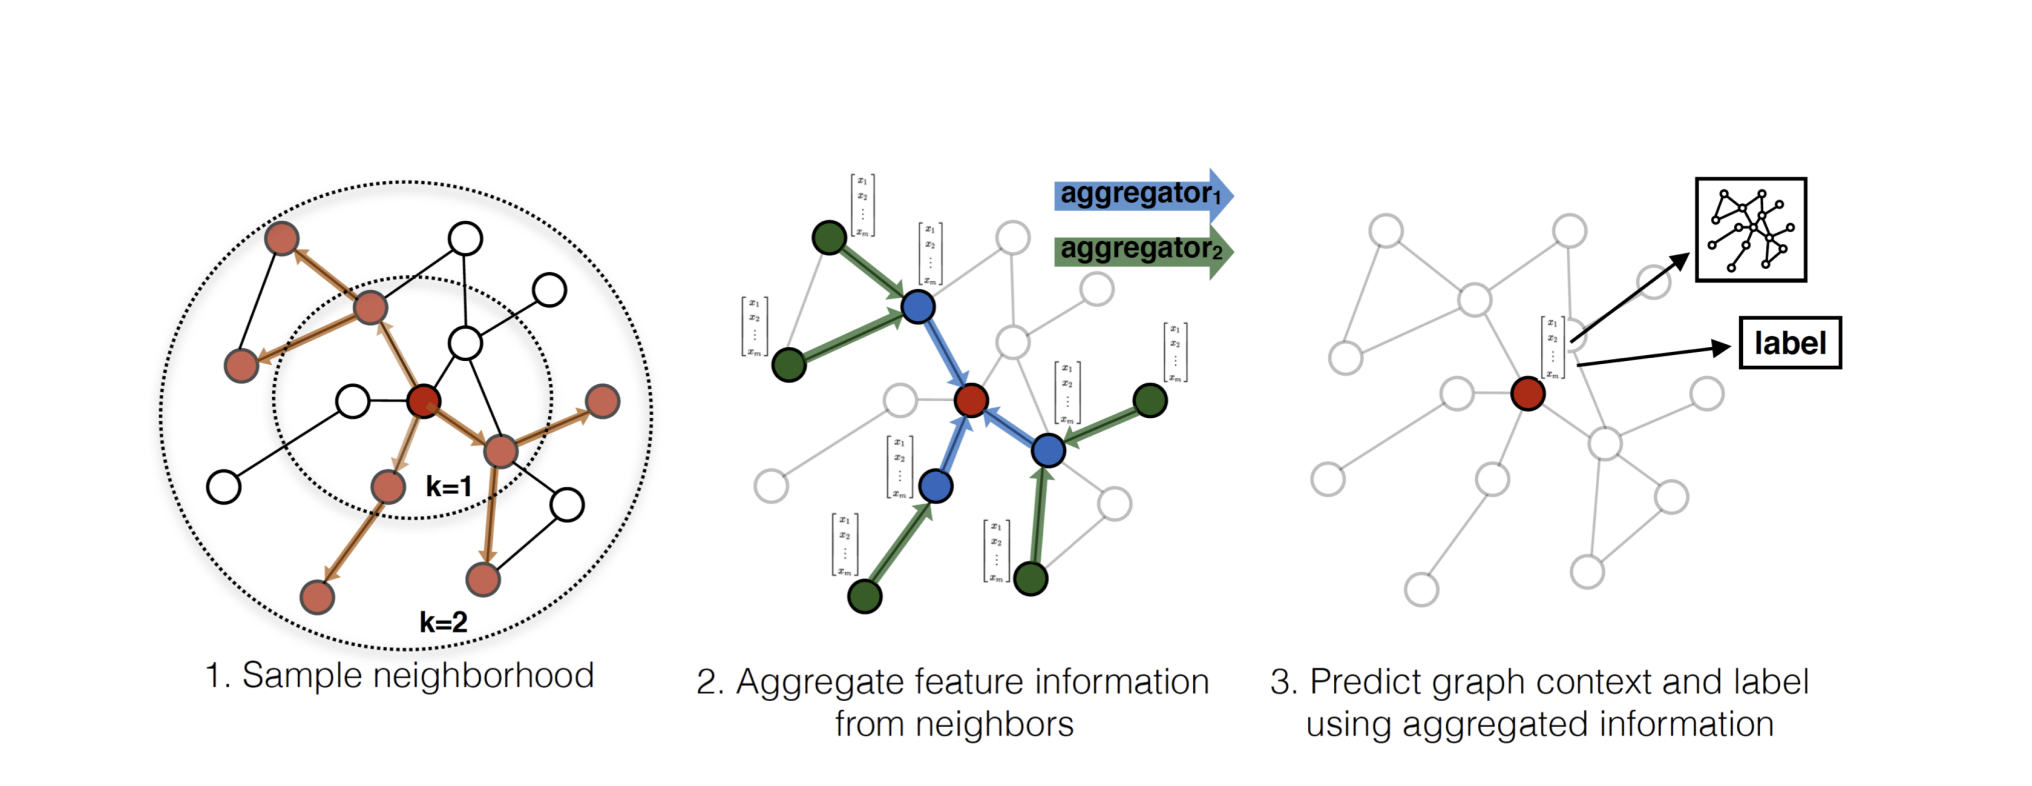
\includegraphics[width=0.8\textwidth]{graphsage.png}
		\caption{GraphSage Sampling}
		\cite[p. 2]{hamilton2017inductive}
		\label{fig:GraphSage_sample}
	\end{figure}

	\noindent The steps shown in figure \ref{fig:GraphSage_sample} are similar
	to the procedures for GCNs. The pseudo code for the GraphSage forward 
	propagation layers is given in algorithm \ref{algo:GraphSage} 
	\cite[p. 12]{hamilton2017inductive}. \\


	\begin{algorithm}[h]
		\scriptsize
		\SetAlgoLined
		\KwIn{Graph $G(V,E)$;}
		\myinput{input features \{$x_v,\forall v \in \mathcal{B}$\};}
		\myinput{depth $K$;} 
		\myinput{weight matrices $W^{k},\forall k \in\{1,\dots,K\}$;}
		\myinput{non-linearity $\sigma$;}
		\myinput{differentiable aggregator functions $AGGREGATE_k,\forall k \in
					\{1,\dots,K\}$;}
		\myinput{neighborhood sampling functions, $\mathcal{N}_k:v\rightarrow
					2^{v},\forall k \in \{1,\dots,K\}$}
		\KwOut{Vector representations $z_v$ for all $v\in\mathcal{B}$}
		\nl $\mathcal{B}^{K}\in\mathcal{B}$\\
		\nl \For{$k=K\dots 1$}{
		\nl		$\mathcal{B}^{k-1}\leftarrow\mathcal{B}^{k}$\\
		\nl		\For{$u\in\mathcal{B}^{k}$}{
		\nl			$\mathcal{B}^{k-1}\leftarrow\mathcal{B}^{k-1}\cup\mathcal{N}_{k}(u)$
					}
				}
		\nl $h_{u}^{0}\leftarrow x_{v},\forall v \in \mathcal{B}^{0}$\\
		\nl \For{$k=1\dots K$}{
		\nl		\For{$u\in\mathcal{B}^{k}$}{
		\nl			$h_{\mathcal{N}(u)}^{k}\leftarrow
					AGGREGATE_k(\{h_{u'}^{k-1},\forall u'\in \mathcal{N}_{k}(u)\})$\;
		\nl			$h_{u}^{k}\leftarrow\sigma\left(W^{k}\cdot
					CONCAT(h_{u}^{k-1},h_{\mathcal{N}(u)}^{k})\right)$\;
		\nl			$h_{u}^{k} \leftarrow h_{u}^{k}/\lVert
					h_{u}^{k}\rVert_{2}$		
				}		
			}
		\nl $z_v \leftarrow h_{u}^{K},\forall u \in \mathcal{B}$
		\caption{GraphSAGE minibatch forward propagation algorithm}
		\label{algo:GraphSage}
	\end{algorithm}
	
	\noindent Note that algorithm \ref{algo:GraphSage} assumes that the
	parameters of the $K$ aggregator functions and the weight matrices $W^{k}$
	are known. Algorithm \ref{algo:GraphSage} thus shows the forward
	propagation of a trained GraphSage model. The model is trained by
	optimizing the model parameters for every batch trained during a specified 
	number of epochs. The training procedure can be implemented by using an
	adaptation of the general procedure shown in algorithm 
	\ref{algo:GNN_struct}. In algorithm \ref{algo:GraphSage} $\mathcal{B}$ 
	refers to the mini-batch training for the set of vertices $V$ of the graph 
	$G(V,E)$. \\

	\noindent There are three aggregator types proposed for GraphSage
	\citep{hamilton2017inductive}:

	\begin{enumerate}
		\item Mean aggregation
		\item Max pooling
		\item LSTM (Long short-term memory) aggregation
	\end{enumerate}

	\noindent The three proposed aggregation strategies are briefly introduced
	as follows: \\

	\noindent\textbf{Mean Aggregation}:\\
	\noindent This type of aggregation is similar to the GCN and takes the
	average of the received messages from the message passing process. The 
	difference to GCN is that mean aggregation does not rely on the full graph 
	Laplacian and makes use of a slightly different normalization approach. The 
	aggregation process differs to the one shown in algorithm 
	\ref{algo:GraphSage} and replaces the procedures in line 9 and 10 with 
	\citep[p. 5]{hamilton2017inductive}:

	\begin{equation}
		h_{v}^{k} \leftarrow \sigma\left(W\cdot
		\text{MEAN}(\{h_{v}^{k-1}\}\cup\{h_{u}^{k-1},\forall u \in \mathcal{N}(v)\})\right)
	\end{equation}

	\noindent\textbf{Max Pooling}:\\
	\noindent Max Pooling aggregation refers to the application of an 
	element-wise $\max$ operator. This means 
	that of the neighbors, only the largest features are considered. More 
	formally, max pooling aggregation is defined as follows and is used for the
	aggregation shown in line 9 of algorithm \ref{algo:GraphSage} 
	\citep[p. 6]{hamilton2017inductive}:

	\begin{equation}
		AGGREGATE_{k}^{pool} = \max\left(\sigma(\{W_{pool}h_{u_{i}}^{k} +
		b),\forall u_{i} \in \mathcal{N}(v)\}\right)
	\end{equation}

	\noindent Note, that $W_{pool}$ refers to a separate weight matrix for the 
	one layer ANN of the max pooling aggregation. In principle, an arbitrary 
	number of layers could be added for max pooling. The authors 
	\cite{hamilton2017inductive} however focus on the case with one layer. The
	parameters of max pooling are learned analogues to the other GraphSage
	model parameters. \\ 

	\noindent\textbf{LSTM}:\\
	\noindent LSTM is the last aggregation strategy proposed for GraphSage and
	uses the LSTM recurrent neural network (RNN) first introduced by
	\cite{hochreiter1997long} as an aggregation strategy. LSTMs are not
	permutation invariant which is a requirement for the aggregation strategy.
	The authors propose using a random permutation of the set of node neighbors 
	to counter this problem \citep[p. 5]{hamilton2017inductive}. The LSTM
	parameters are trained along with the other GraphSage model parameters.  

	\section{Graph Generation}


NWEWEREWFADSFASDFASFAS --- Rewrite

	The MAG model was introduced for
	random graph generation where the feature data is randomly assigned using a
	specified strategy such as Bernoulli trials. This was done, as it is the
	authors aim to find model specifications which create realistic graphs. For
	the purpose of this thesis, this model will be used where the attributes
	correspond to the features in a dataset. This is where the application of
	the model differs in this thesis compared to how it was used in the orginal
	papear. 


	\noindent As mentioned in the introduction, gathering network data
	including features is rather difficult task. This is especially true, as
	most databases do not capture relationships. Further, it is very difficult
	if not impossible to collect network data using standard surveys. This is a 
	problem for this master thesis for which no perfect solution exists. As
	outlined, this problem sparked the research question as to whether network
	data can be generated from cross-sectional data for subsequent and
	meaningful machine learning tasks. Among the many graph generation 
	algorithms researched, the Multiplicative Attribute Graph (MAG) model by 
	\cite{kim2012multiplicative} appears to provide a feasible solution and
	will be used for this thesis. \\

	\noindent The MAG model makes use of two main inputs which are:

	\begin{enumerate}
		\item Node attribute vectors $a_i$
		\item Link-affinity matrices $\Theta_i$
	\end{enumerate}

	\noindent The node attribute vector $a_i$ is part of the graph node-attribute
	generation matrix $B^{N \times K}$. For the purpose of graph generation, 
	only attributes can be considered for which reasonable link-affinity 
	probabilities can be defined. Therefore $B \subseteq X$ where $X^{N \times F}$ 
	is the full feature matrix with $N$ observations and $F$ features. The 
	feature matrix $X$ could for instance be data collected in a survey or a 
	client database with absent relational information. $F$ could for instance 
	refer to the number of questions in a survey for which responses were 
	collected. Every respondent in the survey subsequently is considered as a 
	node in graph setting and the responses are the corresponding node features. 
	Note, that the authors refer to node features as attributes. The terms are 
	used interchangeably for the purpose of this thesis. The $K$ appropriate 
	features which can be included in $B$ are variables for which reasonable
	link-affinity probabilities can be defined. A typical example for this 
	could be age. One could imagine an appropriate setting in which people of 
	the same age group are more likely to form a connection / become friends in 
	a social network setting versus people which are in different age groups. 
	Another example for this could be gender in terms of biological sex which 
	is a classical binary setting for a link-affinity matrix. An example for 
	binary attribute link-affinity matrices $\Theta_i$ is given in figure 
	\ref{fig:link-affinity}.

	\begin{figure}[h]
		\centering
		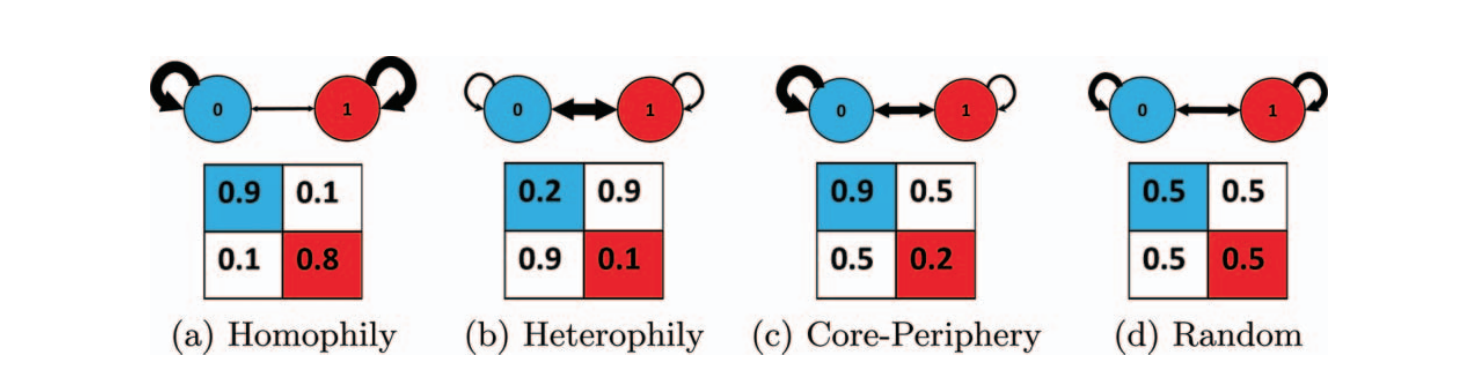
\includegraphics[width=0.8\textwidth]{affinity_matrices.png}
		\caption{Node-attribute link-affinities}
		\cite[p. 118]{kim2012multiplicative}
		\label{fig:link-affinity}
	\end{figure}

	\noindent Figure \ref{fig:link-affinity} shows 4 types of link-affinity
	matrices depending on the relationship between nodes one wants to model.
	Homophily refers to love of the same which would make a connection between
	two nodes more likely if they have the same features. Similarly,
	Heterophily refers to the love of the different where nodes which do not
	have the same features are more likely form a connection. Core-periphery is
	a special case which can be used to generate realistic social-networks in
	terms of network properties \citep[p. 139]{kim2012multiplicative}. For
	instance one could model a group of people in terms of whether they are
	members in a football club or not. It would then be reasonable to assume,
	that members of a football club are very likely to be connected while
	non-members have a significantly lower probability of forming a
	connections. Lastly, random graphs can be generated by setting the
	link-affinity probabilities to 0.5. Given the available data sets, graphs 
	will be generated using homophily structures. The node-attribute
	link-affinity matrices $\Theta_i$ are defined for every attribute and can
	be set for an arbitrary size of categories within an attribute (extends
	beyond the binary setting). More formally for each node $u \in V$ with $K$
	categorical attributes of cardinality $d_i$ for $i = 1,2,\dots,K$ and
	corresponding link-affinity matrices $\Theta_i \in d_i \times d_i$ for
	$i=1,2,\dots,K$, the probability $P[u,v]$ of an edge between nodes
	$(u,v)$ is defined as \citep[p. 119]{kim2012multiplicative}:

	\begin{equation}
		P[u,v] = \prod_{i=1}^{K}\Theta_{i}[a_{i}(u),a_i(v)]
		\label{eq:MAG}
	\end{equation}

	\noindent In equation \ref{eq:MAG} $a_{i}(u)$ refers to the value of the 
	$i$th attribute of node $u$. A schematic representation of the procedure
	for a binary link-affinity matrix is shown in figure \ref{fig:MAG}.

	\begin{figure}[h]
		\centering
		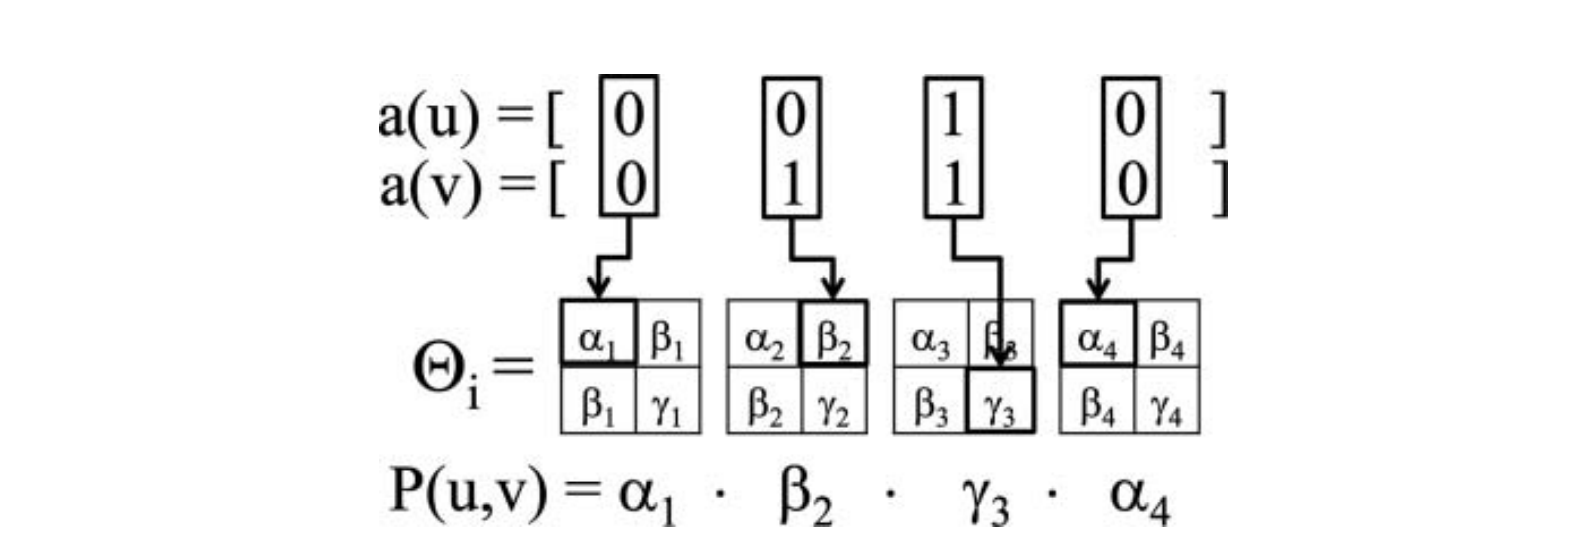
\includegraphics[width=0.8\textwidth]{MAG.png}
		\caption{Schematic representation of the 
			multiplicative attribute graphs (MAG) model}
		\cite[p. 120]{kim2012multiplicative}
		\label{fig:MAG}
	\end{figure}
	

	\begin{algorithm}[h]
		\scriptsize
		\SetAlgoLined
		\KwIn{graph node-attribute generation matrix $B^{N \times K}$, where 
			$B\subseteq X^{N \times F}$;}
		\myinput{node attribute vector $a_i$ with
			cardinalities $d_i$ for $i=1,2,\dots,K$;}
		\myinput{link affinity matrices $\Theta_i \in 
			d_i \times d_i$ for $i= 1,2,\dots,K$;}
		\KwOut{adjacency Matrix $A^{N\times N}$ for Graph $G(V,E)$} 
		\nl $B^{K \times N} = B^{T}$ \\
		\nl \For{$j = 1,2,\dots,N$}{
		\nl	$u = B[:,j]$\\
		\nl		\For{$k = 1,2,\dots,N$}{
		\nl			$v = B[:,k]$\\
		\nl			\For{$i = 1,2,\dots,K$}{
		\nl				$P_{j,k} = \prod_{i=1}^{K}\Theta_{i}[a_{i}(u),a_i(v)]$
						}
				}
			}
		\nl $U^{N \times N} = uppertriangular(P)$ with $diag(U)=0$\\
		\nl \For{$i=1,2,\dots,N$}{
		\nl		\For{$j=1,2,\dots,N$}{
		\nl			\If{$U_{i,j} > \mathcal{U}(0,1)$}{
		\nl				$\hat A_{i,j} = 1$} 
		\nl			\Else{$\hat A_{i,j} = 0$}
				}
			}
		\nl $A = \hat A + \hat A^{T}$

		\caption{Multiplicative Attribute Graph Model}
		\label{algo:MAG}
	\end{algorithm}

	\noindent Algorithm \ref{algo:MAG} generates the adjacency matrix $A$ for
	constructing the resulting graph $G(V,E)$. The node features $X$ can
	thereafter be assigned to the corresponding nodes as the node ordering of 
	the adjacency matrix corresponds to the ordering of the node feature matrix
	$X$. The resulting graph $G(V,E)$ is therefore constructed by first
	assigning the probabilities for two node $(u,v)$ to form a connection based 
	on the link-affinity matrices $\Theta_i$. Once the probabilities are
	calculated, a connection is formed if the probability for a connection is
	larger than a randomly drawn value from a standard uniform distribution
	$\mathcal{U}(0,1)$. If the probability is lower, no connection is formed.
	As this thesis focuses on undirected graphs with no self-edges, the
	resulting adjacency matrix $A$ is symmetric with $diag(A) = 0$. In order to
	ensure this, the upper triangular matrix $U$ of the probability matrix $P$ 
	is taken and setting the $diag(U)=0$. Tis ensures, that the resulting
	adjacency matrix is symmetric and contains no self-edges. 
